\chapter{CERN Laboratories}

\section{Financial and Organizational Sturcutre }

\subsection{Funding Model}

The CERN operating budget provided by the individual member states. The size of the contribution is determined:
\begin{quote}
``using the arithmetic average of three years of Net National
Income values until year before last year and applying the corresponding annual average
exchange rate for each year''
\end{quote}
Here the Net National Income is defined as:

\begin{center}
\begin{table}[]
\begin{center}
\caption{A summary of the GDP, CERN lab contribution, and the ratio between GDP and the absolute contribution 
by country}
\begin{tabular}{cccc}
\textbf{Country} & GDP & Abs (Rel) Cont. & (Cont/GDP) $\times 10^{-7}$ \\
\hline
Germany & \$3.36T  & 231M CHF (20.5\%) & 6.8 CHF/USD  \\
France  & \$2.24T  & 170M CHF (15.1\%) & 7.5 CHF/USD\\
UK      & \$2.86T  & 161M CHF (14.3\%) & 5.6 CHF/USD\\
Italy   & \$1.82T  & 125M CHF (11.1\%) & 6.9 CHF/USD\\
Spain   & \$1.19T  & 88M  CHF (7.82\%) & 7.4 CHF/USD\\
\hline
USA     & \$18.03T & -             & -     \\
\end{tabular}
\end{center}
\label{tab:gdpcontrib}
\end{table}
\end{center}

\begin{center}
\begin{table}[]
\begin{center}
\caption{CMS Gender Demographics by Age as of 2014. Age groups are separated by age range. Each column sums to 100\% of the given gender.
There are a total of4119 Males and 863 females. This corresponds to a global gender ratio of 4.77 men to every 1 female. The ratio is 
between the absolute numbers of men and women within that age range.}
\begin{tabular}{cccc}
\textbf{Age Range} & \textbf{\% of Men} & \textbf{\% of Women} & \textbf{Male/Female Ratio}\\
\hline
$<$ 25 & 12.6\% & 19.4\% & 3.1  \\
25-29 & 20.0\% & 24.0\% & 4.0  \\
30-34 & 12.8\% & 15.0\% & 4.2  \\
35-39 & 9.7 \% & 8.4\%  & 5.0  \\
40-44 & 8.5\%  & 8.3 \% & 4.9  \\
45-49 & 8.3\%  & 7.2 \% & 5.5  \\
50-54 & 8.5\%  & 7.0\%  & 5.8  \\
55-59 & 6.6\%  & 5.0\%  & 6.3  \\
60-64 & 5.2\%  & 2.6\%  & 9.8  \\ 
65-69 & 3.8\%  & 2.1\%  & 8.7  \\
$>$69  & 4.1\%  & 0.6\%  & 34 \\ 
\end{tabular}
\end{center}
\end{table}
\end{center}
 
\begin{center}
\begin{table}[]
\begin{center}
\caption{Differences in Aboslute NNI vs GDP for the year 2015. Countries are ordered by absolute 
contribution size from highest to lowest.}
\begin{tabular}{ccccc}
\textbf{Country} & \textbf{GDP [USD]} & \textbf{NNI [USD]} &  \textbf{NNI/GDP} & \textbf{NNI/Capita}    \\
\hline
Germany & 3.36T & 3.31T & 0.99 & 40.6k\\
France  & 2.24T & 2.27T & 1.01 & 34.4k\\
UK      & 2.86T & 2.33T & 0.81 & 35.8k\\
Italy   & 1.82T & 1.84T & 1.01 & 30.3k\\
Spain   & 1.19T & 1.33T & 1.12 & 28.6k\\
\hline
USA     & 18.03T & 15.67 & 0.87 & 48.7k\\
\end{tabular}
\end{center}
\label{tab:nnicontrib}
\end{table}
\end{center}


\begin{figure}
\begin{center}
%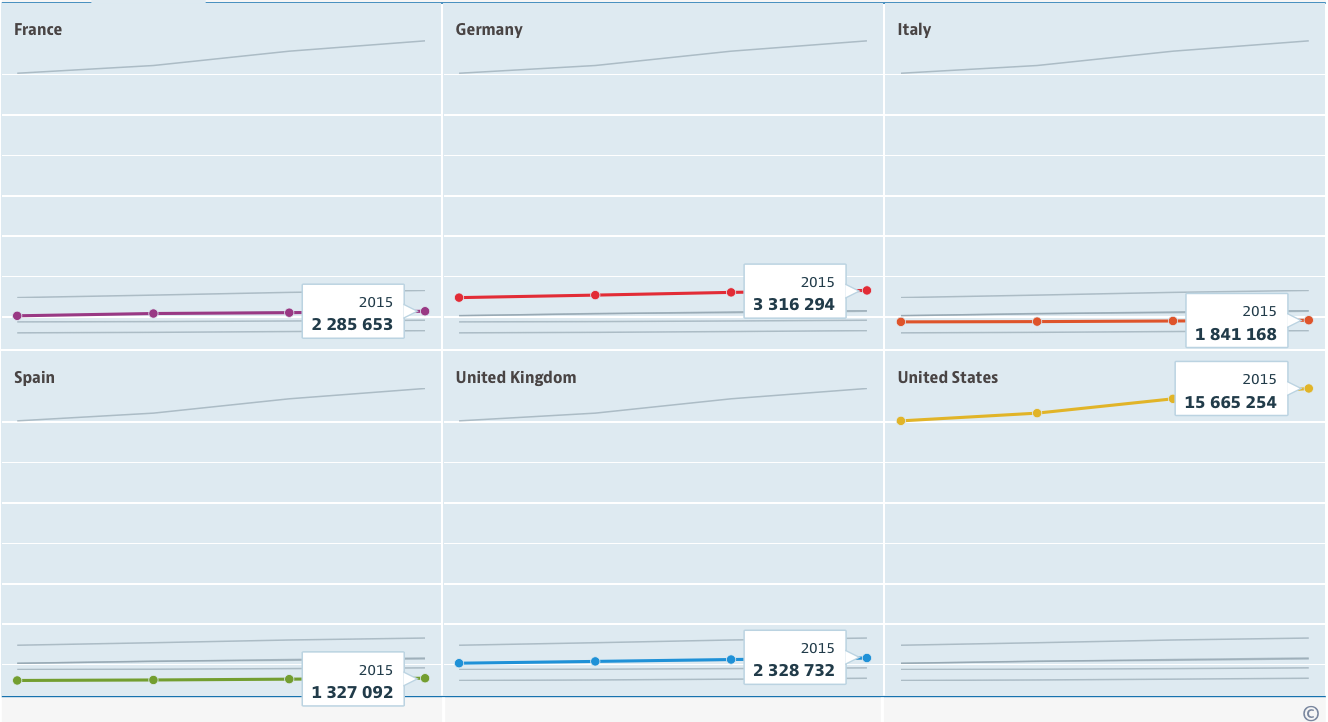
\includegraphics[width=.95\textwidth]{pics/NNI}
\caption{Net National Income for member countries over the three year period used in the average 
generating the 2015 budget for CERN Laboratories}
\end{center}
\end{figure}

\subsection{Organizatiional Structure}



\section{The Large Hadron Collider}

\begin{figure}
\begin{center}
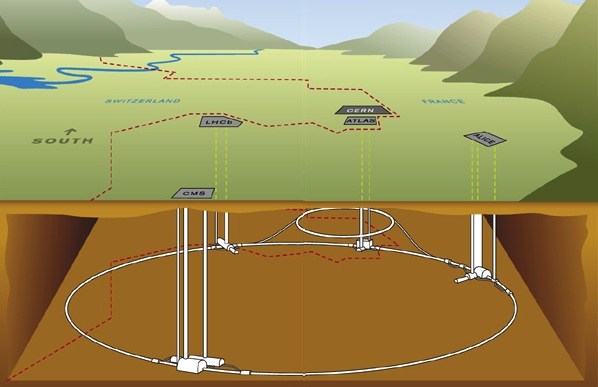
\includegraphics[width=.7\textwidth]{lhc_tunnel}
\caption{The LHC tunnel installed on the border of Geneva, Switzerland and France. 
The experiments are distributed along the circumference of the ring.}
\end{center}
\end{figure}

\begin{figure}
\begin{center}
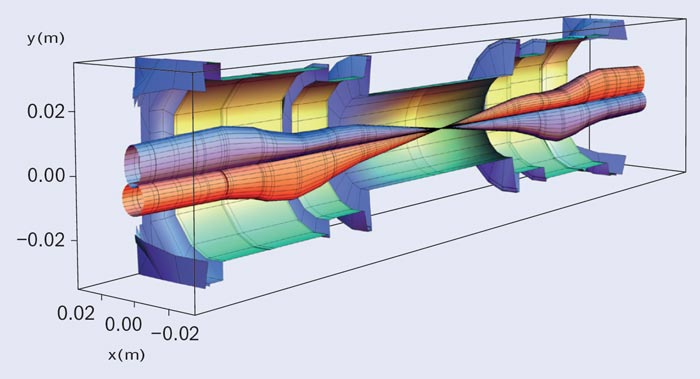
\includegraphics[width=.7\textwidth]{pics/beam_squeeze}
\caption{Squeeze}
\end{center}
\end{figure}


\begin{figure}
\begin{center}
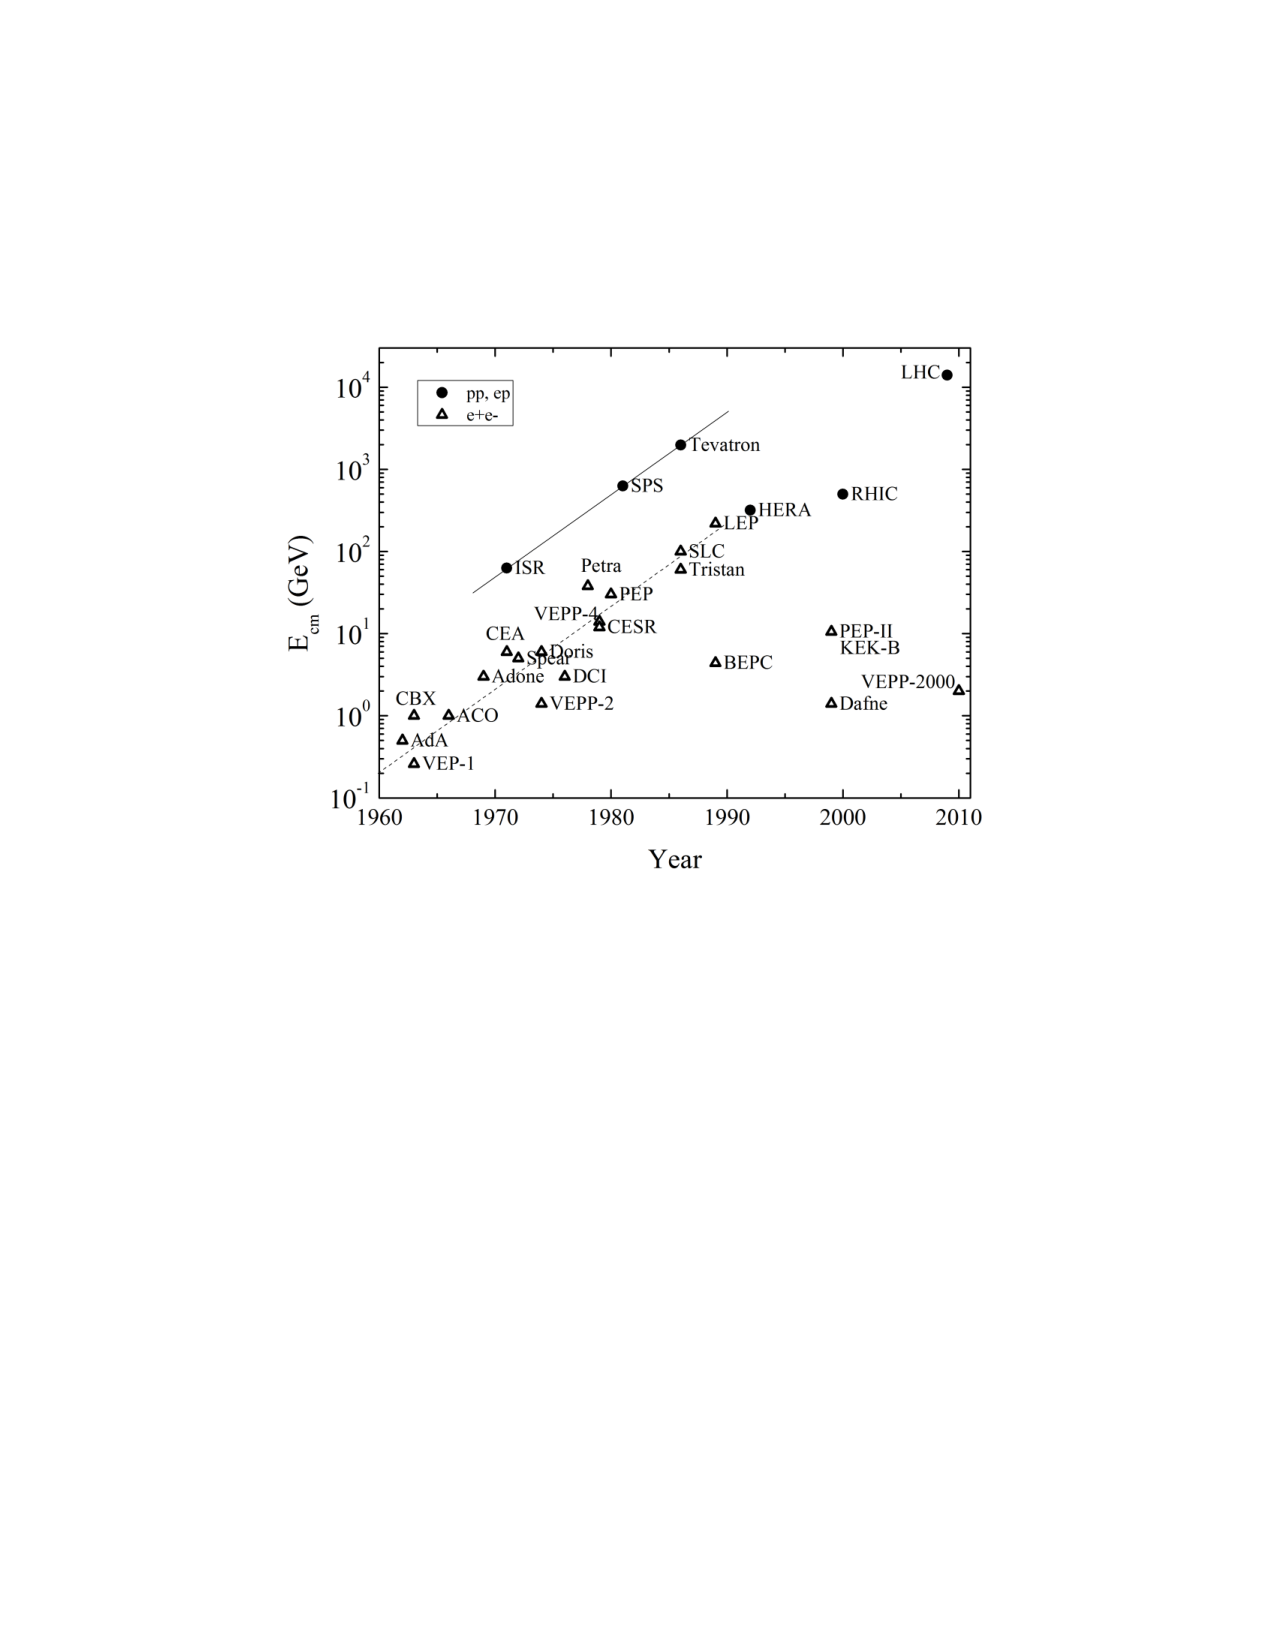
\includegraphics[width=.75\textwidth]{pics/collider_energies}
\caption{Historical Progression of collider energies}
\end{center}
\end{figure}



\begin{figure}
\begin{center}
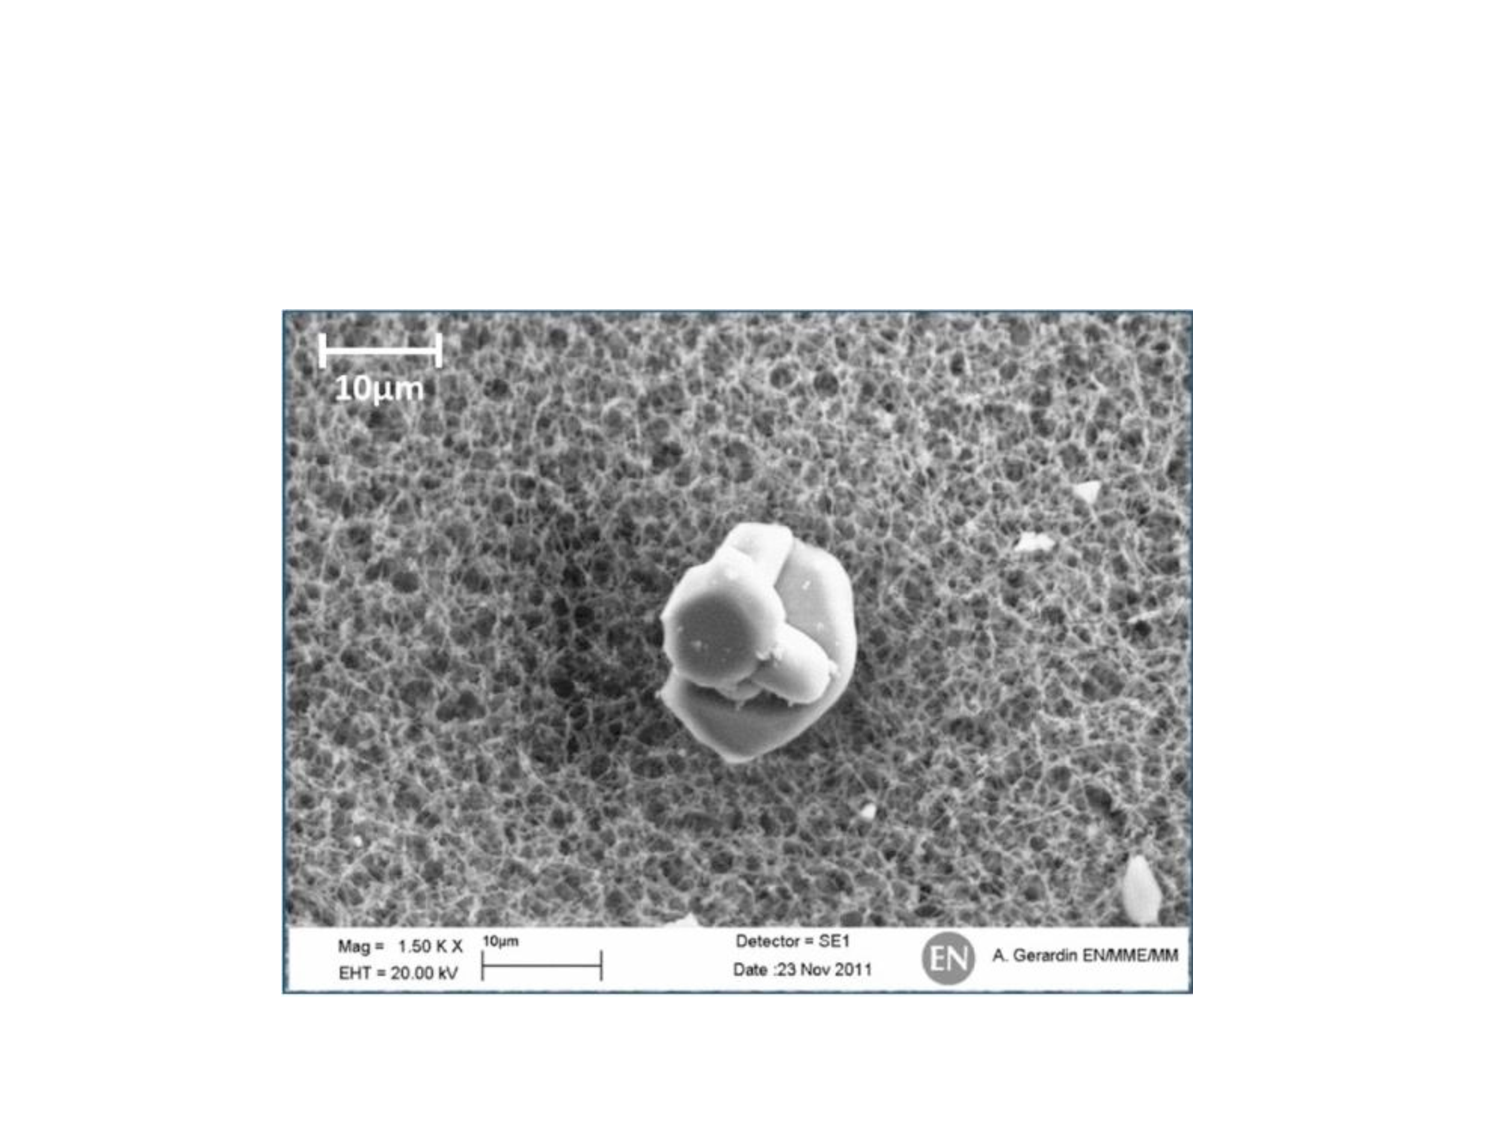
\includegraphics[width=.75\textwidth]{pics/dust}
\caption{Unidentified Falling Objects (UFOs)}
\end{center}
\end{figure}


\begin{center}
\begin{table}[]
\begin{center}
\caption{LHC Running Parameters \cite{lhcparams}}
\begin{tabular}{ccc}
\textbf{Parameter} & \textbf{Value} & \textbf{Remarks} \\
\hline
Circumference (km) & 26.7 km & 100-150 m underground\\
Number of Dipoles & 1232 & Nb-Ti Cables \\
Length of Dipole & 13.3 m & \\
Dipole Field Strength & 8.4 T & Results form high beam energy \\
Operating Temperature & 1.9 K & He cooled superconducting magnets\\
Current in Dipole Coils & 13kA & Results from high magnetic field \\
Beam Intensity & 0.5 A & \\ 
Beam Stored Energy & 362 MJ & 1MJ melts 2kg Cu \\
Magnet Stored Energy / octant & 1100 MJ & \\
\end{tabular}
\end{center}
\end{table}
\end{center}


The bunches of protons in the LHC are bent into a circular trajectory by more than 1200
 superconducting dipole magnets and are focused and maintained close to the ideal
 orbit around the ring by hundreds of superconducting quadrupole magnets. 
Thousands of corrector magnets around the ring allow the beam to be steered closer 
to the ideal orbit, make the focusing independent of the particles’ energy variations
 within a bunch, and cancel the effects of higher order multipoles in the fields induced 
by small field imperfections in the main magnets. 
The radiofrequency (RF) field in superconducting cavities is placed periodically around 
the ring and accelerates the protons from the injection energy of 450 GeV to the final
 operating energy, which is designed to be 7 TeV per beam. The RF field also causes the
 protons to be bunched, as only particles at or near a certain ”equilibrium phase” on 
the RF wave will be accelerated stably. Special quadrupoles around each interaction region
 focus the bunches down to a small transverse size, to increase the likelihood of a
 proton-proton collision each time two bunches pass through each other.
